\documentclass{beamer}
\usepackage{beamerthemesplit}
\usepackage{wrapfig}
\usetheme{SPbGU}
\usepackage{pdfpages}
\usepackage{amsmath}
\usepackage{cmap} 
\usepackage[T2A]{fontenc} 
\usepackage[utf8]{inputenc}
\usepackage[english,russian]{babel}
\usepackage{indentfirst}
\usepackage{amsmath}
\usepackage{tikz}
\usepackage{multirow}
\usepackage[noend]{algpseudocode}
\usepackage{algorithm}
\usepackage{algorithmicx}
\usetikzlibrary{shapes,arrows}
\usepackage{fancyvrb}
\newtheorem{rutheorem}{Теорема}
\newtheorem{ruproof}{Доказательство}
\newtheorem{rudefinition}{Определение}
\newtheorem{rulemma}{Лемма}
\beamertemplatenavigationsymbolsempty

\newtheorem{proposition}[theorem]{Лемма}
\newtheorem{defn}[theorem]{Определение}
\newtheorem{coroll}[theorem]{Следствие}

\title[]{Синтаксический анализ данных, представленных в виде контекстно-свободной грамматики}
\subtitle[]{}
% То, что в квадратных скобках, отображается в левом нижнем углу. 
\institute[СПбГУ]{
Санкт-Петербургский государственный университет \\
Кафедра системного программирования }

% То, что в квадратных скобках, отображается в левом нижнем углу.
\author[Дмитрий Ковалев]{Ковалев Дмитрий Александрович, 444 группа \\
  % У научного руководителя должна быть указана научная степень
  \and  
    {\bfseries Научный руководитель:} к.\,ф.-м.\,н. Григорьев С.\,В. \\ 
  % Для курсовой не обязателен. Должна быть указана должность или ученая степень
  \and
    {\bfseries Рецензент:} программист НИУ ИТМО Авдюхин Д.\,А.}

\date{9 июня 2017 г.}

\definecolor{orange}{RGB}{179,36,31}

\begin{document}
{
% Лого университета или организации, отображается в шапке титульного листа
\begin{frame}
  \begin{center}
  {
\includegraphics[width=1.5cm]{pictures/SPbGU_Logo.png}}
  \end{center}
  \titlepage
\end{frame}
}

\begin{frame}[fragile]
  \transwipe[direction=90]
  \frametitle{Контекстно-свободное сжатие}
  \begin{itemize}
		\item КС-грамматика как компактное представление данных
  \end{itemize}
	\begin{table}
		\begin{tabular}{p{5cm} p{5cm}}
			\begin{center}
				abcabdabcababcabdabcab
			\end{center}
			&
			$$
			\begin{array}{crcl}
			&0 &::=& 1 \, 1 \\
			&1 & ::= & 2 \, d \, 2 \\
			&2 & ::= & 3 \, c \, 3\\
			&3 & ::= & a \, b
			\end{array}
			$$
		\end{tabular}
	\end{table}
	\begin{itemize}
		\item Известные алгоритмы: LZW, Sequitur, Sequential, Re-Pair, ...
		\item Грамматика порождает ровно одну строку (Straight-line grammar)
		\begin{itemize}
			\item отсутствуют рекурсивные вызовы
		\end{itemize}
	\end{itemize}
\end{frame}

\begin{frame}
  \transwipe[direction=90]
  \frametitle{Поиск шаблонов в сжатых данных}
	\begin{itemize}
		\item Поиск шаблонов в КС-представлении без декомпрессии
		\item Шаблон может быть
		\begin{itemize}
			\item строкой (compressed pattern matching)
			\item 'straight-line' грамматикой (fully compressed pattern matching)
			\item регулярным выражением
		\end{itemize}
		\pause
			\item Шаблоны, описываемые КС-грамматикой: 
			\begin{itemize}
				\item поиск рРНК в сжатом геноме
%				\item поиск рРНК в сжатой метагеномной сборке
%				\begin{itemize}
%					\item регулярная грамматика (рекурсивные вызовы)
%				\end{itemize}
			\end{itemize}
	\end{itemize}
\end{frame}

\begin{frame}
	\transwipe[direction=90]
	\frametitle{Синтаксический анализ КС-представления}
	\begin{defn}
		$G_p$, $G_d$ --- произвольные КС-грамматики; $L(G_d) = \{\omega_1, \omega_2, \dots, \omega_k, \dots \}$. Необходимо определить, существуют ли строки $\omega'$, для которых верно: $\omega' \in L(G_p)$ и $\omega'$ --- подстрока одной из строк $\omega_i \in L(G_d)$.
	\end{defn}
	\begin{itemize}
		\item В общем случае задача неразрешима
		\begin{itemize}
			\item сводится к задаче о проверке пустоты пересечения двух КС-языков
		\end{itemize}
	\end{itemize}
\end{frame}

\begin{frame}
  \transwipe[direction=90]
  \frametitle{Постановка задачи}
	\textbf{Целью} данной работы является разработка алгоритма синтаксического анализа данных, представленных в виде контекстно-свободной грамматики. Для ее достижения были поставлены следующие задачи.
	\begin{itemize}
		\item Определить ограничения, при которых синтаксический анализ КС-представления является разрешимой задачей
		\item Разработать алгоритм синтаксического анализа КС-представления данных с учетом поставленных ограничений
		\item Реализовать предложенный алгоритм
		\item Провести экспериментальное исследование
	\end{itemize}
\end{frame}

\begin{frame}
	\transwipe[direction=90]
	\frametitle{Разрешимость задачи}
	\begin{rutheorem}[Nederhof, Satta, 2004 г.]
		Пусть $G_1$ --- произвольная КС-грамматика, $G_2$ --- грамматика, которая не содержит непосредственной или скрытой рекурсий. Тогда проблема проверки $L(G_1) \cap L(G_2) = \emptyset$ относится к классу PSPACE-complete.
	\end{rutheorem}
	\begin{coroll}
		Пусть $G_p$ --- произвольная КС-грамматика, $G_d$ задает конечный язык $L(G_d) = \{\omega_1, \, \dots \, , \omega_n \}$. В таком случае задача синтаксического анализа $G_d$ разрешима и принадлежит PSPACE-complete классу.
	\end{coroll}
\end{frame}

\begin{frame}
	\transwipe[direction=90]
	\frametitle{Рекурсивные автоматы и КС-грамматики}
	\begin{itemize}
		\item Контекстно-свободную грамматику можно представить в виде рекурсивного автомата
		\item На ребрах могут быть как терминальные символы, так и состояния-нетерминалы
	\end{itemize}
		\begin{table}
			\begin{tabular}{p{5cm} p{5cm}}
				\vspace{15pt}
				$$
				\begin{array}{crcl}
				&S' & ::= & S  \\
				&S  & ::= & \texttt{[ } S \texttt{ ]} \\
				&S  & ::= & \texttt{a}
				\end{array}
				$$
				&
				\vspace{-15pt}
				\begin{center}
					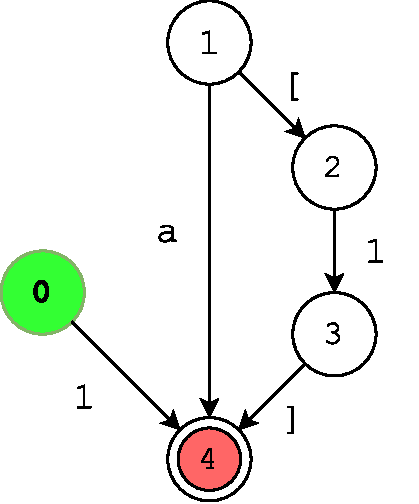
\includegraphics[width=4cm]{pictures/RA}
				\end{center}
			\end{tabular}
		\end{table}
\end{frame}

\begin{frame}
	\transwipe[direction=90]
	\frametitle{Алгоритм}
	\begin{itemize}
		\item \textbf{Вход}:
		\begin{itemize}
			\item $G_p$ --- произвольная КС-грамматика 
			\item $G_d$ --- КС-грамматика без рекурсии, представленная в виде рекурсивного автомата R
		\end{itemize} 
		\item \textbf{Результат}: $\{(n_1, n_2)\}$, где $n_1, n_2$ --- номера состояний автомата $R$, при этом существует $\omega$ такая, что $\omega \in L(G_p)$ и $\omega \in L(R')$, где $R'$ получен из $R$ заменой стартового и конечного состояний на $n_1$, $n_2$
	\end{itemize}
	
\end{frame}

\begin{frame}
	\transwipe[direction=90]
	\frametitle{Реализация}
	\begin{itemize}
		\item Основан на алгоритме обобщенного синтаксического анализа GLL
		\begin{itemize}
			\item позволяет использовать произвольную КС-грамматику
			\item более сложная структура стека (GSS)
		\end{itemize}
		\item Модификация GLL для синтаксического анализа конечных автоматов [Рагозина А., 2016 г.; Горохов А., 2017 г.]
		\begin{itemize}
			\item производит анализ регулярного множества строк, \linebreak представленного автоматом
		\end{itemize}
		\item Основные управляющие функции изменены для поддержки рекурсивных автоматов
		\begin{itemize}
			\item обработка нетерминальных переходов и финальных состояний
			\item два взаимосвязанных GSS
		\end{itemize}
		\item Алгоритм реализован в рамках исследовательского проекта YaccConstructor на F$\#$
	\end{itemize}
\end{frame}

\begin{frame}
	\transwipe[direction=90]
	\frametitle{Эксперименты}
	\begin{itemize}
		\item Последовательность случайных символов
		\item Содержит определенное количество шаблонов, \\ удовлетворяющих грамматике $$S ::= \texttt{[} \, S \, \texttt{]} \, \, | \, \, a$$
		\item Сжатие в КС-грамматику (алгоритм Sequitur)
		\item Для замеров оценивается размер входной грамматики
		$$ |G| = \sum_{p \in P} length(p) $$
	\end{itemize}
\end{frame}


\begin{frame}
	\transwipe[direction=90]
	\frametitle{Эксперименты: время работы}
	Грамматика шаблона: $S ::= \texttt{[} \, S \, \texttt{]} \, \, | \, \, a$
	\begin{center}
		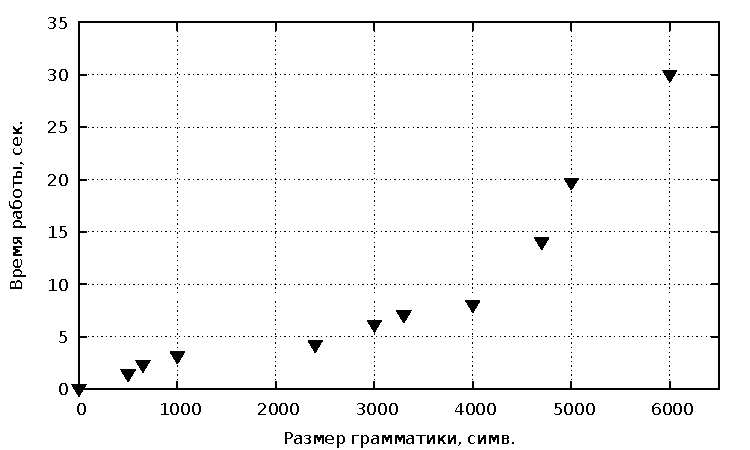
\includegraphics[width=10cm]{pictures/time.pdf}
	\end{center}
\end{frame}

\begin{frame}
	\transwipe[direction=90]
	\frametitle{Эксперименты: память}
	Грамматика шаблона: $S ::= \texttt{[} \, S \, \texttt{]} \, \, | \, \, a$
	
	Измеряется размер стеков (GSS) анализатора
	\vspace{-20pt}
	\begin{table}
		\centering
			\begin{tabular}{p{6cm} p{6cm}}
				\begin{center}
					\hspace{-20pt}
					{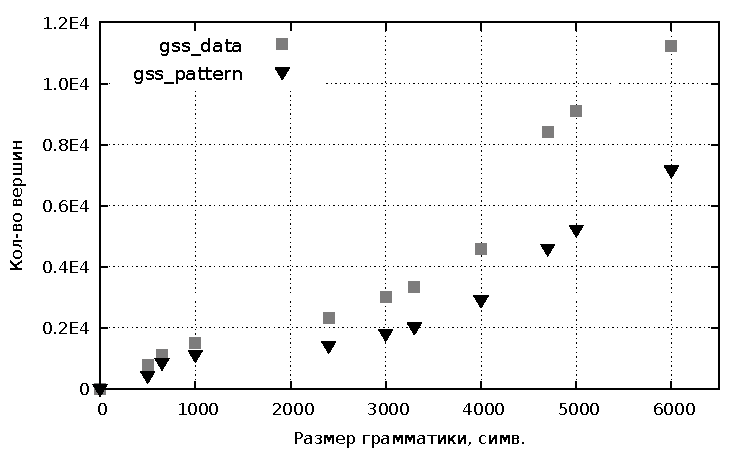
\includegraphics[width=6.2cm]{pictures/gss.pdf}}
				\end{center}
				&
			  \begin{center}
			  	\hspace{-25pt}
			  	{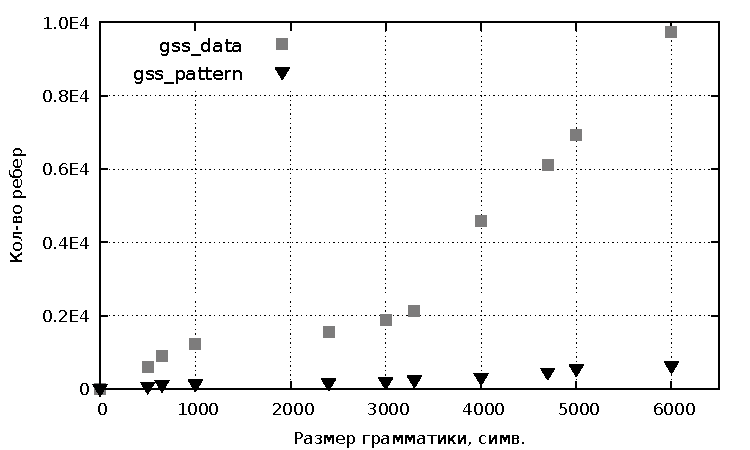
\includegraphics[width=6.2cm]{pictures/gss_edge.pdf}}
			  \end{center}
			\end{tabular}
	\end{table}
Полиномиальный рост объема используемой памяти --- PSPACE
\end{frame}

\begin{frame}
  \transwipe[direction=90]
  \frametitle{Заключение}
	\begin{itemize}
		\item Определены ограничения, при которых синтаксический анализ \\ контекстно-свободного представления является разрешимой задачей
		\item Разработан алгоритм синтаксического анализа КС-представления, учитывающий поставленные ограничения
		\item Предложенный алгоритм реализован на языке программирования F$\#$ в рамках исследовательского проекта YaccConstructor
		\item Проведено экспериментальное исследование
	\end{itemize}
	
	\begin{itemize}
		\item По материалам работы был выполнен доклад на конференции PLC'17, тезисы опубликованы в сборнике материалов конференции. Принята к публикации статья в журнале, входящем в список ВАК.
	\end{itemize}
\end{frame}

\end{document}
